\documentclass[10pt]{beamer}

\usetheme{moloch}

\usepackage{booktabs}
\usepackage[scale=2]{ccicons}

\usepackage{multirow}
\usepackage{pgfplots}

\usepackage{tabularx}

\usepgfplotslibrary{dateplot}
\usepackage{tikzpeople}
\usepackage{tikz}
\usetikzlibrary{overlay-beamer-styles}
\usetikzlibrary{backgrounds}
\usetikzlibrary{shapes}
\usetikzlibrary{shadings}

\usepackage{fontawesome5}
\usepackage{amsmath}
\usepackage{amssymb}

\usepackage{algorithm}
\usepackage{float}
\usepackage{algpseudocode}
% to \uncover a \procedureblock
\usepackage{adjustbox}

\algrenewcommand\algorithmicrequire{\textbf{Input:}}
\algrenewcommand\algorithmicensure{\textbf{Output:}}
\newcommand{\kkk}{\mathbf{k}}
\newcommand{\KKK}{\mathbf{K}}
\newcommand{\rrr}{\mathbf{r}}
\newcommand{\iNTT}{$\mathsf{iNTT}$}
\newcommand{\bch}{\mathsf{BCH}}
\newcommand{\intt}{\mathsf{iNTT}}
\newcommand{\leap}{\textsc{Leap}}
\usepackage{xcolor}
\definecolor{mBGcol}{HTML}{fafafa}
\definecolor{colA}{HTML}{990099}
\definecolor{colC}{HTML}{b6b6b6}
\definecolor{colB}{HTML}{00b300}
\definecolor{colD}{HTML}{2eb8b8}
\definecolor{thirdColor}{HTML}{6A5ACD}


\newcommand{\bv}[1]{\mathbf{#1}}
\usepackage[lambda,landau,operators,probability,sets,logic,advantage,complexity,asymptotics,notions,mm,primitives,ff,adversary,advantage]{cryptocode}


\title{Oblivious Transfer, Extended}
\subtitle{Oblivious Evaluations for Privacy}
\date{9$^{th}$ of June, 2026}
\author{Lena Heimberger}
\institute{QSCAN 2026, Vienna}
\titlegraphic{\hfill
\includegraphics[height=1cm]{figures/logo.pdf}}
\pgfplotsset{compat=1.18}

\begin{document}

\maketitle

\begin{frame}{Hi, I'm Lena}
  \begin{columns}[T]
    \column{0.7\textwidth}
      \textbf{Who I am}
      \begin{itemize}
        \item PhD student @ Graz University of Technology 
        \item Privacy in a Post-Quantum World \pause
      \end{itemize}
      \vspace{0.8em}
      \textbf{This talk}
      \begin{itemize}
        \item Two OT-based protocols
        \item A Pseudorandom Function~(PRF)
        \item Put them together: \leap
      \end{itemize}
    \column{0.3\textwidth}
      \begin{tikzpicture}[>=stealth, font=\small,
                          node distance=1.1cm]
        \node[draw, rounded corners=4pt,
              fill=mLightGreen!15, text=mDarkTeal,
              minimum width=3cm, align=center] (ot)
              {OT $+$ OLE};
        \node[draw, rounded corners=4pt,
              fill=mLightGreen!15, text=mDarkTeal,
              minimum width=3cm, align=center,
              below of=ot] (prf)
              {\textsc{Spring} PRF};
        \node[draw, rounded corners=4pt,
              fill=mLightBrown!15, text=mDarkTeal,
              minimum width=3cm, align=center,
              font=\bfseries\small,
              below of=prf] (leap)
              {$\mathsf{Leap}$};
        \draw[->] (ot.south)  -- (prf.north);
        \draw[->] (prf.south) -- (leap.north);
      \end{tikzpicture}
  \end{columns}
\end{frame}

\section{Two Protocols to start the two-party computation}
\begin{frame}
  \frametitle{$n\choose 1$-OT}
  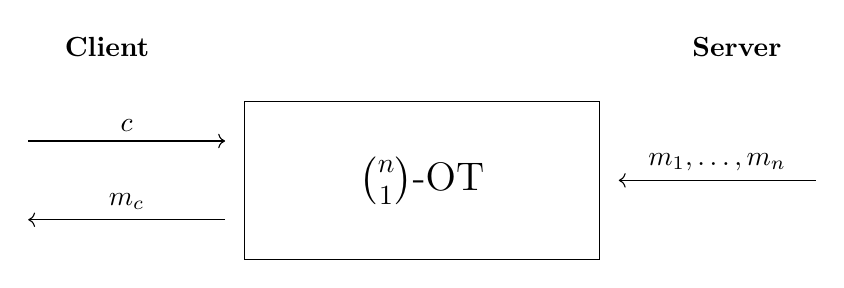
\begin{tikzpicture}
    \node[text centered] at (-4, 1.7) {\textbf{Client}};
    \node[text centered] at (4, 1.7) {\textbf{Server}};

    \node[draw, text centered, minimum width= 4.5cm, minimum height=2cm] at
      (0,0){\Large{$n\choose 1$-OT}};
    \draw[->](5, 0) -- (2.5, 0)node[midway,above]{$m_1, \ldots, m_{n}$};

    \draw[->] (-5, 0.5)  -- (-2.5, 0.5) node[midway,above]{$c$};
    \draw[->] (-2.5, -0.5) -- (-5, -0.5) node[midway,above]{$m_{c}$};
  \end{tikzpicture}
  %   \vspace{1em}
  %   Generic construction from \alert{${\log q}$ $2\choose 1$-OTs} !

\end{frame}

\begin{frame}{$n\choose 1$-OT from $\log n$ OTs}
  \begin{tikzpicture}[>=stealth, thick, font=\small]

    %% ── Parameters ──────────────────────────────────────────────────
    %% Suppose q = 2^k, so log q bits. We draw k = 4 OT boxes for concreteness.
    \def\nbits{4}         % number of 2-choose-1 OTs shown
    \def\boxw{1.1cm}
    \def\boxh{1.5cm}
    \def\xstep{2.0}       % horizontal spacing between OT boxes

    %% ── Alice and Bob (tikzpeople) ──────────────────────────────────
    \node[chef, hat=black, female, hair=violet, shirt=black, minimum size=1.2cm,
      label={[font=\bfseries\small]above:Alice}] (alice) at (-4, 0) {};

    \node[sailor, mirrored, minimum size=1.2cm,
      label={[font=\bfseries\small]above:Bob}]   (sailor)   at (5.5,  0) {};

    %% ── Alice's input label ─────────────────────────────────────────
    \node[font=\footnotesize, text=mDarkTeal, above=0.05cm of alice] (xlab) {};
    \node[font=\footnotesize, text=mDarkTeal, below=0.55cm of alice]
      {$c = c_0 c_1 c_2 c_3$};

    %% ── OT boxes ────────────────────────────────────────────────────
    \foreach \i in {0,1,2,3} {
      \pgfmathsetmacro{\xpos}{\i * \xstep}
      \node[draw, rounded corners=3pt,
        minimum width=\boxw, minimum height=\boxh,
        font=\footnotesize\bfseries,
        label={[font=\scriptsize, text=mDarkTeal!40]below:bit $\i$}]
        (ot\i) at (\xpos - 2, 0)
        {$2\choose 1$-OT};

      %% Alice sends bit c_i into each box
      \draw[<-, mDarkTeal, thin]
        (ot\i.north west) ++(0.0,0.0) -- ++(0, 0.7)
        node[above, font=\scriptsize, text=mDarkTeal] {$c_{\i}$};

      %% Bob sends two messages into each box
      \draw[<-, red!60!black, thin]
        (ot\i.north east) ++(0.0, 0.0) -- ++(0, 0.7)
        node[above, font=\scriptsize, text=red!60!black]
        {$d^{(\i)}_0, d^{(\i)}_1$};
    }
    % 
    %% ── Ellipsis between last real box and "final" box ───────────────
    \node[font=\large] at (3*\xstep + 1.0, 0) {$\cdots$};

    %% ── Combine outputs → final result ─────────────────────────────
    \node[draw, rounded corners=5pt, fill=blue!10,
      minimum width=2.0cm, minimum height=0.9cm,
      font=\footnotesize\bfseries, text=mDarkTeal]
      (combine) at (\xstep - 1, -2.2)
      {combine};

    %% Arrows from each OT box down to combine
    \foreach \i in {0,1,2,3} {
      \draw[->, mDarkTeal!40, thin] (ot\i.south) -- (combine.north);
    }
    %   \draw[->, mDarkTeal!40, thin] (otlast.south) -- (combine.north);

    %% ── Output label ────────────────────────────────────────────────
    \draw[->] (combine.south) -- ++(0, -0.8)
      node[below, font=\footnotesize, text=mDarkTeal]
      {$d_c = d_{c_0}^{(0)}\oplus d_{c_1}^{(1)}\oplus d_{c_2}^{(2)} \oplus d_{c_3}^{(3)}$};

    % %% ── Complexity callout ──────────────────────────────────────────
    % \node[draw=orange!50, fill=orange!5, rounded corners=4pt,
    %       font=\scriptsize, text=orange!80!black,
    %       text width=3.2cm, align=center]
    %       at (3*\xstep + 2.5, -2.2)
    %       {$\lfloor \log q \rfloor$ \;OTs\\[2pt]
    %        instead of $n = q$ messages};
  \end{tikzpicture}
\end{frame}

\begin{frame}{Agreeing on a flat}
  \begin{exampleblock}{Motivating example}
    Alice and Bob are  looking for a new flat. Depending on the location, they only want to pay a certain amount of rent per room, but neither want to put down concrete numbers.
  \end{exampleblock}\pause
  \begin{columns}[T]
    \column{0.3\textwidth}
    \hspace{-5em}
    \begin{figure}
      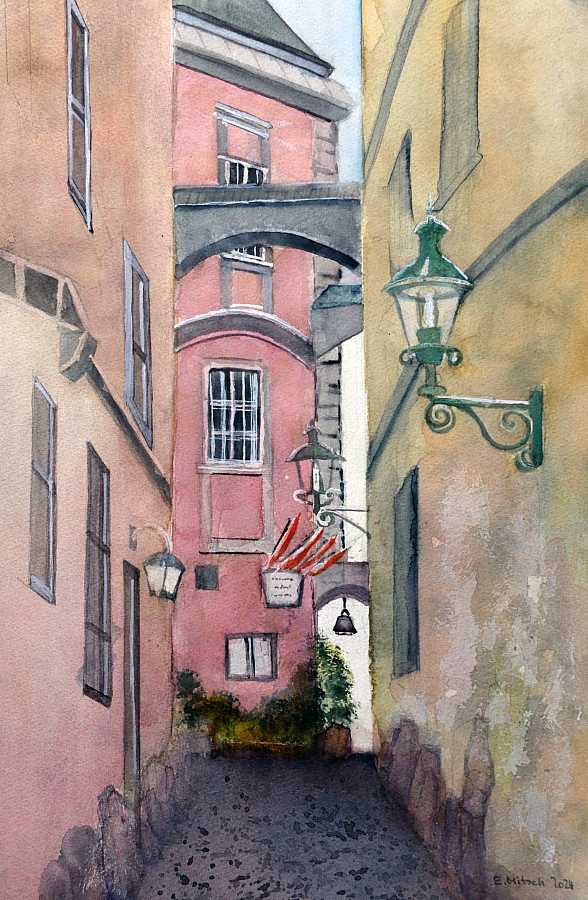
\includegraphics[scale=0.2]{figures/altbau.jpg}
    \caption{\tiny{\url{https://www.aquarell.me/bilder/oesterreich/wien}}}
    \end{figure}
    \pause

    \column{0.32\textwidth}
    \begin{figure}
      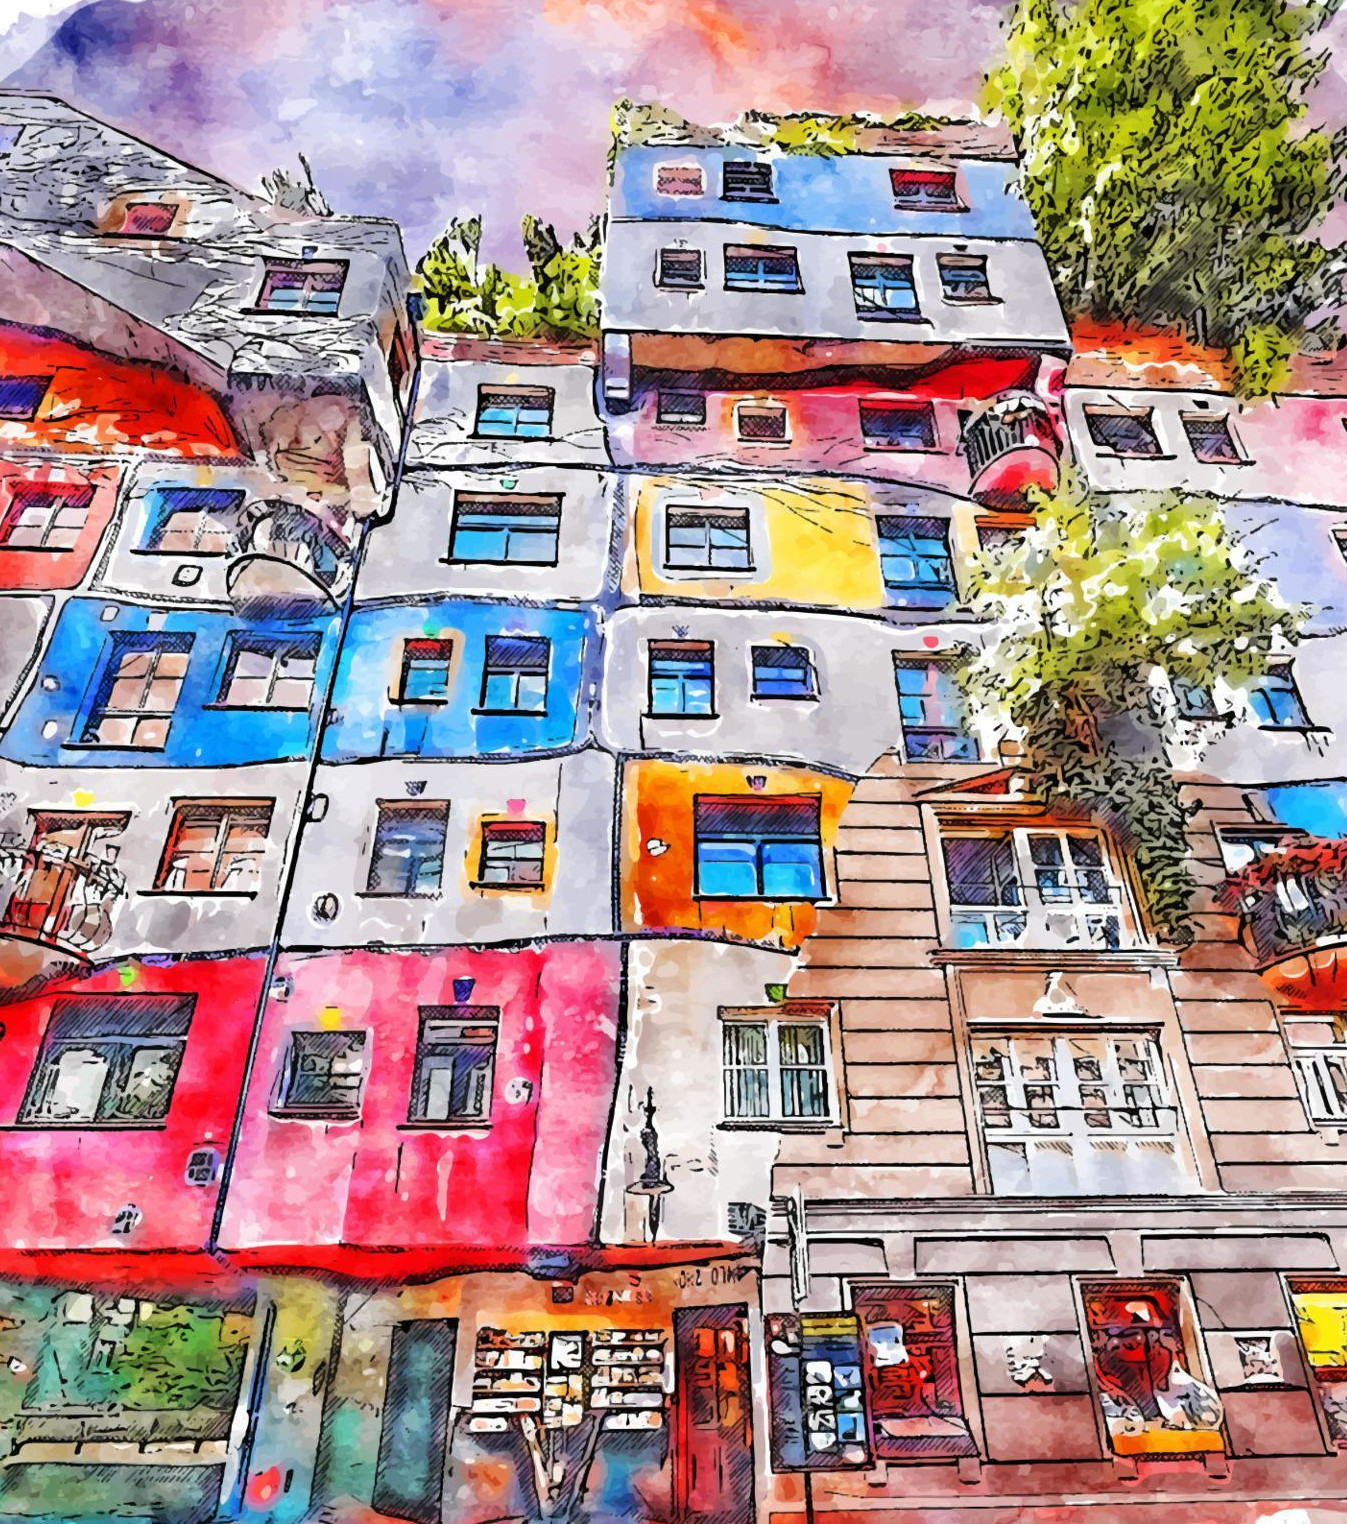
\includegraphics[scale=0.37]{figures/neubau.jpg}
    \caption{\tiny{\url{https://de.vecteezy.com/vektorkunst/12911197-wien-osterreich-aquarell-skizze -handgezeichnete-illustration}}}
    \end{figure}
    \pause

    \column{0.32\textwidth}
    \begin{figure}
      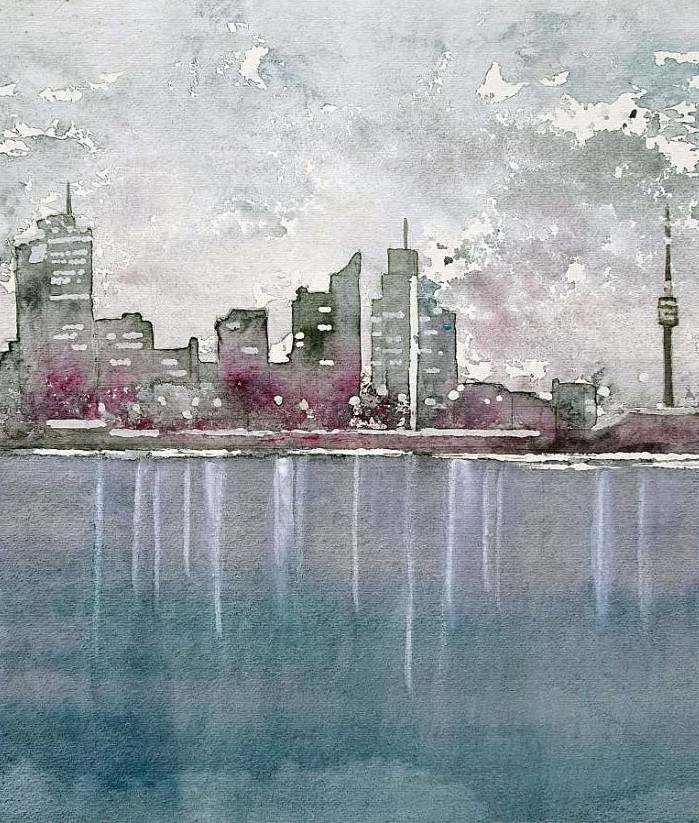
\includegraphics[scale=0.22]{figures/transdanubien.jpg}
    \caption{\tiny{\url{https://www.aquarell.me/bilder/oesterreich/wien}}}
    \end{figure}
  \end{columns}
\end{frame}

\begin{frame}{Obliviously rounding two values $\mod q$}
  \begin{tikzpicture}[>=stealth, thick, font=\small]

    %% Alice (left)
    \node[chef, hat=black, female, hair=violet, shirt=black, minimum size=1.4cm,
      label={[font=\bfseries]above:Alice}] (alice) at (-4.5, 0) {};

    %% Bob (right)
    \node[sailor, mirrored, minimum size=1.4cm,
      label={[font=\bfseries]above:Bob}] (sailor) at (4, 0) {};

    %% Input labels beneath characters
    \node[font=\footnotesize, text=mDarkTeal, below=0.4cm of alice]
      {holds $a \in \mathbb{Z}_q$};
    \node[font=\footnotesize, text=violet, below=0.4cm of sailor]
      {holds $b \in \mathbb{Z}_q$};

    %% Arrow with label — node is part of the draw command
    \draw[<-] (alice.east) -- (sailor.west)
      node[midway, above, text=red!60!black,
      text width=5cm, align=center, font=\scriptsize]
      {$\lfloor a_i + b \rceil \oplus\, d_{a_i}$\\
      $\forall\, a_i \in \mathbb{Z}_q$};

    %% Privacy annotation — Alice
    \node[draw=mLightGreen, fill=blue!5, rounded corners=4pt,
      font=\scriptsize, text=mDarkTeal,
      text width=2.8cm, align=center]
      at (-4.5, -2.4)
      {learns $\lfloor a + b \rceil$ only\\[2pt]
      {\color{mDarkTeal!40}$b$ stays hidden}};

    %% Privacy annotation — Bob (x-coord matches Bob at 4)
    \node[draw=red!30, fill=red!5, rounded corners=4pt,
      font=\scriptsize, text=red!70!black,
      text width=2.8cm, align=center]
      at (4, -2.4)
      {learns nothing about\\[2pt]$a$};

  \end{tikzpicture}
  \pause
  \begin{exampleblock}{Example}
    The first apartment costs 800 Euros to rent. \pause Bob is willing to pay 400. His inputs to the OT are 0, 0, 0, 1, 1, 1, for Alice's choices of \{1,2,3,4,5,6)(00) Euros per month.
  \end{exampleblock}
  \alert{
    \pause Generalizes for small value spaces!
  }
\end{frame}
\section{Beyond Simple Arithmetic}

\begin{frame}{Two Telescopes, One Detection}
  \begin{exampleblock}{Motivating example}
    Two radio telescopes record signals $\mathbf{a}, \mathbf{b} \in \mathbb{Z}_q^n$
    independently. To confirm a detection, they need the correlation
    $\langle \mathbf{a}, \mathbf{b} \rangle$, but neither wants to
    expose their raw signal.
  \end{exampleblock}
  \pause
  \vspace{0.5em}
  \begin{tikzpicture}[>=stealth, thick, font=\small]
    \node[chef, hat=black, female, hair=purple, shirt=black, minimum size=1.4cm,
      label={[font=\bfseries]above:Alice}] (alice) at (-4, 0) {};
    \node[sailor, mirrored, minimum size=1.4cm,
      label={[font=\bfseries]above:Bob}] (sailor) at (4, 0) {};

    \node[font=\footnotesize, text=mDarkTeal, below=0.4cm of alice]
      {signal $\mathbf{a} \in \mathbb{Z}_q^n$};
    \node[font=\footnotesize, text=red!60!black, below=0.4cm of sailor]
      {signal $\mathbf{b} \in \mathbb{Z}_q^n$};

    \node[draw, rounded corners=6pt, fill=gray!8,
      minimum width=3cm, minimum height=1.6cm,
      font=\normalsize\bfseries] (goal) at (0, 0)
      {$\langle \mathbf{a}, \mathbf{b} \rangle = ?$};

    \draw[->] (alice.east) -- (goal.west);
    \draw[->] (sailor.west)   -- (goal.east);

    \node[draw=mLightGreen!60, fill=mLightGreen!8, rounded corners=4pt,
      font=\scriptsize, text=mDarkTeal,
      text width=2.8cm, align=center]
      at (-4, -2.2)
      {learns $\langle \mathbf{a}, \mathbf{b}\rangle$\\[2pt]
      {\color{gray!60}$\mathbf{b}$ stays hidden}};

    \node[draw=red!30, fill=red!5, rounded corners=4pt,
      font=\scriptsize, text=red!70!black,
      text width=2.8cm, align=center]
      at (4, -2.2)
      {learns nothing\\[2pt]about $\mathbf{a}$};
  \end{tikzpicture}
\end{frame}

\begin{frame}{Oblivious Linear Evaluation (Gilboa \cite{C:Gilboa99})}
      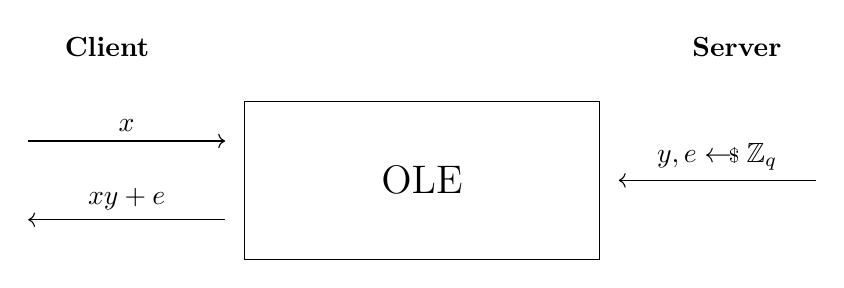
\begin{tikzpicture}
        \node[text centered] at (-4, 1.7) {\textbf{Client}};
        \node[text centered] at (4, 1.7) {\textbf{Server}};
        \node[draw, text centered, minimum width= 4.5cm, minimum height=2cm] at
          (0,0){\Large{OLE}};
        \draw[->](5, 0) -- (2.5, 0)node[midway,above]{$y, e\sample \ZZ_q$};
        \draw[->] (-5, 0.5)  -- (-2.5, 0.5) node[midway,above]{$x$};
        \draw[->] (-2.5, -0.5) -- (-5, -0.5) node[midway,above]{$xy+e$};
      \end{tikzpicture}

      \vspace{1em}
      \begin{block}{}
        \centering
        Client learns $xy + e$\\
        Server learns nothing about $x$\\
        Client learns nothing about $y$ or $e$
      \end{block}
\end{frame}


\begin{frame}{Oblivious Linear Evaluation}
  \begin{itemize}
    \item The correlation $\langle \mathbf{a}, \mathbf{b} \rangle = \sum_i a_i b_i$
      involves \alert{products of private values} --- hard to compute jointly
      \pause
    \item OLE converts one such product into \alert{additive shares}:
      \begin{align*}
        \text{Alice gets } y_i = a_i b_i + e_i, \qquad
        \text{Bob keeps } e_i
      \end{align*}
      Neither learns the other's input \pause
    \item Summing over $i$ gives additive shares of the full inner product:
      \begin{align*}
        \underbrace{\sum_i y_i}_{\text{Alice}} -
        \underbrace{\sum_i e_i}_{\text{Bob}}
        = \langle \mathbf{a}, \mathbf{b} \rangle
      \end{align*}
      \pause
    \item Additive shares are \alert{linear}: easy to mask, rerandomize,
      and feed into the next step
  \end{itemize}
\end{frame}

\section{How is this useful? }

% Brief intro to OPRFs: what they are and why we care
\begin{frame}
  \frametitle{Have you ever wanted to...}
  \begin{itemize}
    \item $\ldots$ send a secret over a wire?\pause
    \item $\ldots$ intersect a set privately?\pause
    \item $\ldots$ take your low-entropy input and get a high-entropy output?
  \end{itemize}
\end{frame}

% Real-world motivation: Why PSI matters for contact discovery, private databases, threat intelligence sharing
\begin{frame}
  \frametitle{You may want to consider an OPRF!}
  \begin{tikzpicture}[every node/.style={minimum width=1.5cm},scale=0.8]

    \node[chef, hat=black, hair=purple, monitor, shirt=black, minimum size=1.5cm, label=Client] (alice)
      {};
    \node[scale=2.67, label=Server, xshift=3.5cm] (server) {{\large{\faServer}}};
    \node[scale=2.67, label=compute, xshift=1.9cm] (hashfunction) {\({y
      \coloneqq F_k(x)}\)};

    \node(Alicetext) [below of=alice,xshift=1cm, yshift=-0.8cm,text
      width=3cm, text=gray]{input \(x \in \mathcal{X}\), gets \(y\)};
    \node(Servertext) [below of=server, xshift=0.5cm,yshift=-0.5cm,text
      width=3cm,text=gray]{key \(k\in \mathcal{K}\)};;
  \end{tikzpicture}
\end{frame}


\begin{frame}
  \frametitle{Pseudorandom Functions \cite{C:GolGolMic84,GolGolMic86} }
  \begin{itemize}
    \item deterministic and polynomial time function $y=F(x,k)$\pause
    \item hard to distinguish output $y$ from a randomly chosen element from
      $y'\in\mathcal{Y}$.
  \end{itemize}\pause
  \begin{exampleblock}{Naor-Reingold PRF}
    \begin{itemize}
      \item Naor-Reingold PRF~\cite{NaoRei04}: built from an Abelian group action $*$\pause
      \item Sample $g_0, \ldots, g_m$; compute $g_0 * \prod_{i=1}^m g_i^{x_i}$\pause
      \item \emph{hashes to group} for free\pause
    \end{itemize}
  \end{exampleblock}
  \begin{example}[Naor-Reingold with seven input bits]
    For example, for $0110111$ we would
    compute the group action $g_0*g_2*g_3*g_5*g_6*g_7$.
  \end{example}
\end{frame}

\begin{frame}{From Elliptic Curves to Lattices}
  \begin{columns}[T]
    \column{0.32\textwidth}
    \begin{exampleblock}{Elliptic curves}
      $F_k(x) = P_0 \sum_{i=1}^m x_i P_i$\\[6pt]
      Algebraic structure hidden
      by ECDLP \checkmark
      \alert{Broken} in presence of a quantum adversary
    \end{exampleblock}\pause

    \column{0.32\textwidth}
    \begin{exampleblock}{Subset products}
      $F_k(x) = g_0 \prod_{i=1}^m g_i^{x_i}\mod p$\\[6pt]
      \alert{Broken}:  multiplicative
      structure is exploitable
    \end{exampleblock}\pause

    \column{0.32\textwidth}
    \begin{exampleblock}{Rounded products}
      $F_k(x) = \left\lfloor g_0\prod_{i=1}^m
      g_i^{x_i} \right\rceil \mod q$\\[6pt]
      Post-quantum \checkmark\\
      \ldots needs careful rounding!
    \end{exampleblock}\pause
  \end{columns}

  \vspace{1em}
  \centering
  Rounding kills the algebraic structure,
  but how do we round \emph{obliviously}?

\end{frame}

\begin{frame}{\textsc{Spring} is a subset-product-based PRF}
  \begin{itemize}
    \item 2014: \alert{heuristic} PRF with using polynomial subset-products with small modulus\pause \\
      $q\in \{257,514\}$\pause
    \item non-heuristic variant: huge $q$! \pause\\ but we're working on it\pause
    \item \cite{EC:HKLMRR25} focus in \textsc{Spring-BCH}: rounding bias reduction using extended BCH code
      $[128,64,22]$\pause
  \end{itemize}

  \onslide<3-6>{
    \begin{figure}[H]
      \label{Spring:PRF}
      \vspace{-1em}
      \begin{align*}
        \mathcal{F}_{\bv{K}}(c_1,
        \cdots,c_m)=S\left(\kkk_0 \prod_{i=1}^m \kkk_{i}^{c_i}\right)
      \end{align*}
    \end{figure}
  }

  \onslide<7>{
    \begin{figure}[H]
      \label{Spring:PRF-intt}
      \vspace{-8em}
      \begin{align*}
        \mathcal{F}_{\bv{K}}(c_1,
        \cdots,c_m)=S\left(\intt\left(\kkk_0\odot \prod_{i=1}^m \kkk_{i}^{c_i}\right)\right)
      \end{align*}
    \end{figure}
  }

  \onslide<8>{
    \begin{figure}[H]
      \label{Spring:PRF-intt-lookup}
      \vspace{-8em}
      \begin{align*}
        \mathcal{F}_{\bv{K}}(c_1,
        \cdots,c_m)=S\left(\intt\left(\mathsf{lookup}\left(\kkk_0+
        \sum_{i=1}^m {c_i}\kkk_{i}\right)\right) \right)
      \end{align*}
    \end{figure}
    Multiplication is addition of exponents! \\
    \vspace*{-1em}
    \begin{align*}
      g^ag^b= g^{a+b}~\text{for some generator $g$}
    \end{align*}
  }
\end{frame}

% \begin{frame}{Why $q=\{257\}$?}
%   \begin{itemize}
%     \item Choice of modulus from ease of implementation:
%     \item $q=257$
%       \begin{itemize}
%         \item only use \emph{invertable} polynomials \pause \\
%         \item Computation mod $q$: use units (nonzero coefficients) \pause \\
%           avoid zeroing out
%         \item Fermat's Theorem for prime $q$:
%           \begin{align*}
%             g^{q-1}\equiv g^0 \equiv 1 \mod q
%           \end{align*}\pause
%         \item use subset-sum of exponents instead of multiplication \pause
%         \item Sample in exponent form $\mod q-1= 256$\pause \\
%           fits in a single byte!
%       \end{itemize}
%   \end{itemize}
% \end{frame}


\begin{frame}{An OPRF from \textsc{Spring}}
  \begin{columns}
    \hspace*{0.1em}
    \vspace*{-3em}
    \begin{column}{.48\textwidth}
      \begin{figure}
        \begin{align*}
          \only<1-2>{
            \color{colC}S\left(\intt\left(\mathsf{lookup}\left(\color{black}\kkk_0+
            \sum_{i=1}^m {c_i}\kkk_{i}\color{colC}\right)\right)\right)
          }
          \only<3-5>{
            \color{colC}S\left(\intt\left(\color{black}\mathsf{lookup}\left(\kkk_0+
            \sum_{i=1}^m {c_i}\kkk_{i}\right)\color{colC}\right)\right)
          }
          \only<6-7>{
            \color{colC}S\left(\color{black}\intt\left(\mathsf{lookup}\left(\kkk_0+
            \sum_{i=1}^m {c_i}\kkk_{i}\right)\right)\color{colC}\right)
          }
          \only<8->{\color{black}
            S\left(\intt\left(\mathsf{lookup}\left(\kkk_0+ \sum_{i=1}^m {c_i}\kkk_{i}\right)\right)\right)
          }
        \end{align*}
      \end{figure}
    \end{column}
    \begin{column}{.67\textwidth}
      \centering
      \vspace*{-3em}
      \resizebox{\textwidth}{!}{
        \begin{tikzpicture}[background rectangle/.style={fill=mBGcol}, show
          background rectangle]
          % Label for Client on the left and Server on the right
          \uncover<1->{
            \node[text centered] at (-4, 2) {\textbf{Client}};
            \node[text centered] at (-4, 1.4) {$\bv{c}=[c_1, \ldots, c_m] \in
              \{0,1\}^m$};
            \node[text centered] at (4, 2) {\textbf{Server}};
            \node[text centered] at (4, 1.4) {$\bv{K}=[\kkk_0, \kkk_1, \ldots, \kkk_m] \in
              \{0,1\}^m$};

            \node[draw, text centered, minimum width= 4.5cm, minimum height=2cm] at
              (0,0){\Large{$2\choose 1$-OT}};
            \draw[->](5, 0) -- (2.5, 0)node[midway,above]{$\bv{r}_i, \bv{r}_i+\kkk_i$};

            \draw[->] (-5, 0.5)  -- (-2.5, 0.5) node[midway,above]{$c_i$};
            \draw[->] (-2.5, -0.5) -- (-5, -0.5) node[midway,above]{$\bv{r}_i+\kkk_i{c_i}$};

          }
          \uncover<2->{
            \draw[line width=0.1 mm] (-5.5,-1.1) -- (5.5,-1.1);
            \node[ text centered, minimum width= 4.5cm, minimum height=1cm] at
              (0,-1.5){$\sum_{i=1}^\kappa \bv{r_i}+c_i \bv{k_i}$\qquad  \qquad\qquad\qquad
              $\kkk_0-(\sum_{i=1}^\kappa \bv{r}_i)$};
          }
          \uncover<3->{
            \node[ text centered, minimum width= 4.5cm, minimum height=1cm] at
              (0,-1.8){\faRecycle};
            \draw[line width=0.2 mm] (-5.5,-2.8) -- (5.5,-2.8);
            \node[ text centered, minimum width= 4.5cm, minimum height=1cm] at
              (0,-2.3){$\bv{b}\leftarrow\prod_{i=1}^\kappa \bv{r_i}\bv{k_i}^{c_i}$\qquad  \qquad\qquad\qquad
              $\bv{a}\leftarrow\kkk_0(\prod_{i=1}^\kappa \bv{r}_i)^{-1}$};
          }
          \uncover<4->{

            \node[draw, text centered, minimum width= 4.5cm, minimum height=2cm] at
              (0,-4){\Large{OLE}};
            \draw[->](-5, -3.6) -- (-2.5, -3.6) node[midway,above]{$b_i$};
            \draw[<-](-5, -4.5) -- (-2.5, -4.5)node[midway,above]{$y_i=a_ib_i+e_i$};
            \draw[<-] (2.5, -4)  -- (5, -4) node[midway,above]{$a_i,
                e_i \sample
              \ZZ_q$};

            \draw[line width=0.1 mm] (-5.5,-5.1) -- (5.5,-5.1);
          }
          \uncover<5->{
            \node[ text centered, minimum width= 4.5cm, minimum height=1cm] at
              (-0.5,-5.5){$\bv{y}\leftarrow\sum_{i=0}^{n-1} (a_i\cdot b_i + e_i) X^i$\qquad \qquad  \qquad\quad
              $\bv{e}\leftarrow\sum_{i=0}^{n-1} e_i X^i$};
          }
          \uncover<6->{
            \node[ text centered, minimum width= 4.5cm, minimum height=1cm] at
              (0,-6){$\intt$};
          }
          \uncover<7->{
            \node[ text centered, minimum width= 4.5cm, minimum height=1cm,
              visible on=<9->] at
              (0.1,-6.5){\qquad\qquad\qquad\qquad\qquad\qquad\qquad\qquad
              $\bv{d}\sample\{0,1\}^n$};
            \draw[line width=0.2 mm] (-5.5,-7) -- (5.5,-7);
          }
          \uncover<8->{
            \node[draw, text centered, minimum width= 4.5cm, minimum height=2cm] at
              (0,-8.5){\Large{$q\choose 1$-OT}};

            \draw[->](-5, -8) -- (-2.5, -8) node[midway,above]{$y_i$};
            \draw[<-, visible on=<8>](-5, -9) -- (-2.5, -9) node[midway,above]{$\lfloor
              y_i-e_i\rceil_p$};
            \draw[<-, visible on=<9->](-5, -9) -- (-2.5, -9) node[midway,above]{$\lfloor
              y_i-e_i\rceil_p\oplus d_i$};
            \draw[->, visible on=<8>](5, -8.5) -- (2.5, -8.5) node[midway,above]{$\lfloor
              (q_i-e_i)\rceil_p $} ;
            \draw[->, visible on=<9->](5, -8.5) -- (2.5, -8.5) node[midway,above]{$\lfloor
                (q_i-e_i)\rceil_p\oplus d_i
              $} ;
            \node [text centered] at (4, -9){$ \forall q_i\in \ZZ_q$};
          }
          \uncover<9->{
            \draw[<-, visible on=<9->](-4, -10.25) -- (4, -10.25)
              node[midway,above]{$\mathsf{BCH(\bv{d})}$};
          }
        \end{tikzpicture}

      }
    \end{column}
  \end{columns}
\end{frame}



\begin{frame}
  \frametitle{Conclusion}
  \begin{itemize}
    \item Generic primitives, composed carefully, give us efficient
      and provably secure protocols 
    \item Ongoing: tighter reductions, smaller parameters,
      stronger security arguments
    \item Many open problems- happy to discuss!
  \end{itemize}
  \hfill \texttt{lena.heimberger@tugraz.at}


\end{frame}
\maketitle


\begin{frame}[allowframebreaks]
  \frametitle{References}

  \bibliography{bilbio,export/crypto,export/abbrev3}
  \bibliographystyle{alpha}

\end{frame}

\begin{frame}{All OT is precomputed}
  \begin{tabularx}{\textwidth}{lllllll}
    \toprule
    \#&\textbf{Protocol} & \multicolumn{2}{c}{\textbf{Communication}} &  \multicolumn{2}{c}{\textbf{Computation}} \\
      & & Client & Server & Client & Server \\
      \midrule
    \multirow{4}{*}{$2^0$}   & Simplest OT+IKNP &39 kB & \textbf{4 kB} & 63 ms &
    63 ms \\
                             & Kyber OT+IKNP & 465 kB & 328 kB &
    \textbf{10 ms} & \textbf{10 ms} \\
                   & Simplest OT+Silent & \textbf{22 kB} & 22 kB &68 ms & 68 ms \\
                   & Kyber OT+Silent & 448 kB& 392 kB& \textbf{10 ms}& 10 ms\\
                   \midrule
                   \multirow{4}{*}{$2^{13}$}
                   & Simplest OT+IKNP & 319 MB & \textbf{4.26 kB} & 420 ms& 463 ms\\
                   & Kyber OT+IKNP & 319 MB& 328 kB&  \textbf{311 ms}&
                   \textbf{423 ms}\\
                   & Simplest OT+Silent & \textbf{46 kB} & 155 kB& 2065 ms& 3371 ms\\
                   & Kyber OT+Silent & 487 kB & 559 kB &2130 ms &3496 ms \\
                   \bottomrule
  \end{tabularx}
  \pause
  \alert{ The OT is interchangable!}
\end{frame}



\begin{frame}{Performance }
  \resizebox{\textwidth}{!}{%
    \begin{tabularx}{\textwidth}{@{}lXXXXcr@{}}
      \toprule
      \multirow{2}{*}{\textbf{Phase}} & \multicolumn{3}{c}{\textbf{Client}} &
      \multicolumn{3}{c}{\textbf{Server}} \\
                                      & Comm. & Comp.  & Idle & Comm. & Comp.  & Idle \\
                                      \midrule
      Subset-Sum & 16 bytes & 5 $\mu$s &21 $\mu$s  & 16\,384 bytes &  863 $\mu$s & 46 $\mu$s \\
      OLE & 144 bytes & 4 $\mu$s  & 3 $\mu$s& 1\,296 bytes  &  72 $\mu$s &88 $\mu$s  \\
      Rounding & 144 bytes & 2 $\mu$s &726 $\mu$s & 4\,118 bytes & 814 $\mu$s & 67 $\mu$s\\
      BCH & 0 bytes&  1 $\mu$s&  0 $\mu$s& 8 bytes& / & 26 $\mu$s \\
      \midrule
      Overall      & 304 bytes&\multirow{2}{*}{11 $\mu$s} &  \multirow{2}{*}{750 $\mu$s}&
      21\,806 bytes& \multirow{2}{*}{ 1.7 ms } &\multirow{2}{*}{227 $\mu$s}\\
      (Network)    & (328 bytes)&  &  &  (22\,840 bytes)&  &\\
      \bottomrule
    \end{tabularx}
  }
\end{frame}

\begin{frame}
  \centering
  \resizebox{\textwidth}{!}{
    \begin{tabular*}{1.6\textwidth}
      {
        @{\extracolsep{\fill}}
        ccccccc
        @{}
      }
      %{cllllll}
      \toprule
&  \multicolumn{2}{c}{Parameters }& \multicolumn{2}{c}{Setup} &
\multicolumn{2}{c}{Online} \\
& $|S|$ & $|C|$ &  $|S|$ & $|C|$&  $|S|$ & $|C|$ \\
\midrule
{\multirow [c]{6}{*}{
{\textbf{\leap} (IKNP+Kyber)}}}
&\multirow [c]{2}{*}{$2^0   $} & \multirow [c]{2}{*}{$2^0$   }& 1 ms & 1 ms&
0.2s
& 6 ms \\
& && 117 bytes & 0 bytes& 73.4 kiB  & 20 KiB\\
&\multirow [c]{2}{*}{$2^5   $} & \multirow [c]{2}{*}{$2^{5}$ }& 1 ms & 1 ms &
  0.08 s & 0.07 s\\
         & & &246 bytes &0 bytes &  802 kiB & 47.5 kiB \\
         &\multirow [c]{2}{*}{$2^{10}$} & \multirow [c]{2}{*}{$2^{10}$}& 4 ms & 5 ms
         &2.4 s & 2.46 s\\
         & & &4.30 kiB &0 bytes &22.39 MiB & 646.5 kiB \\
         \midrule
         {\multirow [c]{6}{*}{
         NR-OT~(FHE OT)~\cite{ASIACCS:HHMRR24}}}
         &\multirow [c]{2}{*}{$2^0   $} & \multirow [c]{2}{*}{$2^0$   }&0.26 s  & 0.51 s &
  0.06 s&
  0.10 s \\
        & & &134 bytes & 1 byte& 128 kiB& 0.75MiB\\

        &\multirow [c]{2}{*}{$2^5   $} & \multirow [c]{2}{*}{$2^{5}$ }& 1.63 s& 1.88 s &
  3.11 s& 3.15 s\\
        & &&263 bytes  & 1 byte &4MiB & 8.5 MiB \\
        &\multirow [c]{2}{*}{$2^{10}$} & \multirow [c]{2}{*}{$2^{10}$}&45.04 s & 45.28 s &
  99.66 s &99.71 s \\
          & & &4.31 MiB & 1 byte & 128 MiB& 256.6 MiB\\
          \midrule
          {\multirow [c]{6}{*}{
          OPUS~\cite{ASIACCS:HHMRR24}}}
          &\multirow [c]{2}{*}{$2^0   $} & \multirow [c]{2}{*}{$2^0$   }& 0.26 s&
  0.26 s &15.47 s& 15.91 s \\
         & & &133 bytes &0 bytes & 17.07 kiB &  9.04 kiB\\
         &\multirow [c]{2}{*}{$2^5   $} & \multirow [c]{2}{*}{$2^{5}$ }&8.71 s &
  8.71 s& 328.46 s & 329.14 s\\
        & & & 262 bytes& 0 bytes & 546.25 kiB& 290.26 kiB \\
        &\multirow [c]{2}{*}{$2^{10}$} & \multirow [c]{2}{*}{$2^{10}$}& 303.38 s &
  303.38 s& 16367.12 s & 16367.60 s\\
          & & &4.31 kiB & 0 bytes & 34.14 MiB & 18.08 MiB \\
          \midrule
          {\multirow [c]{6}{*}{
          ECNR (Simplest OT + IKNP)~\cite{USENIX:KRSSW19}}}
          &\multirow [c]{2}{*}{$2^0   $} & \multirow [c]{2}{*}{$2^0$   }& 10 ms & 0 s&0.23 s
          & 0.05 s \\
          & && 133 bytes & 0 bytes&12.04 kiB  & 16 bytes \\
          &\multirow [c]{2}{*}{$2^5   $} & \multirow [c]{2}{*}{$2^{5}$ }&0.02 s &0 s & 0.21 s& 0.06 s\\
          & & &262 bytes &0 bytes & 137.05 kiB & 512 bytes \\
          &\multirow [c]{2}{*}{$2^{10}$} & \multirow [c]{2}{*}{$2^{10}$}& 0.3 s & 0 s &0.64 s & 0.57 s\\
          & & &4.36 kiB &0 bytes &4.04 MiB &16 kiB \\
          \bottomrule
\end{tabular*}
}
\end{frame}



\end{document}
